\subsection{Структура программного обеспечения и функции его компонентов}\label{sec:software-structure-components}
Программное обеспечение системы включает в себя:
\begin{itemize}
  \item непосредственно программу-редактор~--- SVE: Simple VHDL Editor;
  \item утилиту GHDL~--- симулятор VHDL.
\end{itemize}

Назначение SVE, как компонента системы очевидно: с ее помощью осуществляется создание и редактирование файлов, осуществляется загрузка и сохранение данных, ведется управление расширениями.

GHDL, используемый как бинарный исполняемый файл, выполняет следующие цели:
\begin{itemize}
  \item с программной точки зрения, GHDL может компилировать двоичные файлы на основе исходного кода на VHDL;
  \item с аппаратной точки зрения, GHDL предоставляет средства анализа и симуляции описанной на VHDL системы;
\end{itemize}

В системе используются возможности GHDL по созданию подсветки синтаксических конструкций и проверке корректности (компилируемости) создаваемых программных решений.


\subsection{Выбор компонентов программного обеспечения}

\subsubsection{Операционная система}
Поскольку разработка ведется с использованием кроссплатформенных компонентов, гарантируется работоспособность системы на следующих операционных системах:
\begin{itemize}
  \item Microsoft Windows (начиная с Windows XP);
  \item Linux-дистрибутивы, такие как Debian, Gentoo, Slackware, Ubuntu Linux и др.
  \item Mac OS X;
  \item FreeBSD, OpenBSD и ряд других UNIX-систем.
\end{itemize}

При этом, на каждой из указанных ОС гарантируется выполнение системой всех заявленных функций.

\subsubsection{Инструментальное средство разработки и язык программирования}
На этапе подготовки к разработке актуален вопрос выбора инструментария разработки.
Поскольку поставлена задача разработки сложной системы, выбор необходимо производить, отталкиваясь от связки <<язык программирования -- фреймворк -- IDE>>.

Изначально для достижения наибольшей производительности было принято решение отказаться от дополнительных прослоек между ОС и программной системой.
В силу профессиональных навыков автора, доступности справочной информации и из соображений оптимального соотношения <<поставленные цели -- затраченное время>>, было решено остановиться на С-подобных языках.

Таким образом, при выборе языка и среды разработки рассматривались:
\begin{itemize}
  \item C\# или C++ и Visual Studio от компании Microsoft;
  \item С++ и Code::Blocks, open source-решение;
  \item С++ и Qt Creator от компании Trolltech (Digia) \cite{about-qt}.
\end{itemize}

\small
\singlespacing
\begin{longtable}[h]{|p{0.3\textwidth}|p{0.2\textwidth}|p{0.2\textwidth}|p{0.2\textwidth}|}
  \caption{Сравнение языков программирования и сред разработки}
	\\ \hline
	  \textbf{Критерий}                                              &
	  \textbf{Visual Studio}                                         &
	  \textbf{Code::Blocks}                                          &
	  \textbf{Qt Creator}
	\\ \hline
  \endfirsthead

  \multicolumn{4}{r}{\normalsize Продолжение таблицы \thetable{} \small}
  \\ \hline
    \textbf{Критерий}                                              &
	  \textbf{Visual Studio}                                         &
	  \textbf{Code::Blocks}                                          &
	  \textbf{Qt Creator}
    \\ \hline
  \endhead

  Язык программирования &
  C\#, C++              &
  C++                   &
  C++
  \\ \hline

  Фреймворк &
  .NET      &
  stdLib    &
  Qt
  \\ \hline

  Компоненты разработки графических приложений   &
  Windows Forms, Windows Presentation Foundation &
  wxWidgets                                      &
  QWidgets
  \\ \hline

  Кроссплатформенность &
  нет                  &
  да (Windows, Linux)  &
  да (Windows, Linux, Mac OS X)
  \\ \hline

  Стоимость  &
  19443 руб. &
  бесплатно  &
  бесплатно
  \\ \hline

  Лицензия      &
  проприетарная &
  GNU/GPL       &
  GNU/GPL
  \\ \hline

  Поддержка со стороны разработчика &
  да                                &
  нет                               &
  да
  \\ \hline

\end{longtable}
\normalsize
\onehalfspacing

На основе указанных критериев в качестве языка разработки выбран С++ в связке с программным фреймворком Qt.
Выбор именно этих компонентов обусловлен следующими факторами:
\begin{itemize}
  \item Большое количество готовых компонентов и решений.\\
  Qt предоставляет ряд компонентов, расширяющих или по-своему реализующих компоненты языка C++: QVector (аналог std::vector), QList (аналог std::list), QString (аналог std::string), ряд классов для работы с XML-деревьями, классы для работы с файловой системой и др.
  Использование этих компонентов значительно упрощает разработку за счет наличия большого количества методов, реализующих стандартные методы.
  Более того, использования структур данных Qt зачаствую позволяет добиться преимущества в скорости работы: так, QVector при использовании в Qt-приложениях по скорости выполнения операций выборки и помещения данных выгоднее std::vector \cite{qt}.
  \item Наличие средств разработки пользовательского интерфейса.\\
  Помимо структур данных Qt предоставляет набор компонентов для создания экранных форм и элементов управления (QWidgets): окна, кнопки, текстовые и графические метки, поля ввода, списки, графические области и др.
  Используя эти компоненты, а также встроенный механизм событий и сигналов, можно построить приложение с привлекательным развитым графическим интерфейсом, способствующим решению поставленных задач \cite{qt-creator}.
  \item Переносимость создаваемых решений.\\
  Qt является кроссплатформенным фреймворком~--- с его помощью можно разрабатывать и запускать написанное ПО в большинстве современных операционных систем путем простой компиляции программы для каждой ОС без изменения исходного кода.
  Среди поддерживаемых ОС~--- Windows, Linux, Mac OS X, Android и др. UNIX-подобные.
\end{itemize}

В качестве среды разработки, исходя из ранее выбранного фреймворка, используется Qt Creator.
QtCreator~--- кроссплатформенная свободная IDE для разработки на С, С++ и QML. Разработана Trolltech (Digia) для работы с фреймворком Qt.
Включает в себя графический интерфейс отладчика и визуальные средства разработки интерфейса как с использованием QtWidgets, так и QML.

Использование Qt Creator позволяет облегчить, в первую очередь, проектирование графического интерфейса приложения и написание кода, а во-вторых, централизованно управлять разрабатываемым проектом~--- вести контроль версий, манипулировать ресурсами.

Помимо среды разработки, актуальным инструментом при разработке является система контроля версий.
Она позволяет хранить несколько версий одного и того же документа, при необходимости возвращаться к более ранним версиям, определять, кто и когда сделал то или иное изменение.
В качестве системы контроля версий был выбран Git за его высокую производительность, продуманные команды.
Исходный код разрабатываемой системы распространяется свободно и содержится в публичном репозитории на Github~--- веб-сервисе для хостинга IT-проектов.


\subsection{Разработка прикладного программного обеспечения}

\subsubsection{Структура прикладного программного обеспечения}

Структура ПО системы приведена на рисунке \ref{fig:components-big}.
\begin{figure}[H]
  \centering
  \includegraphics[width=0.9\textwidth]{diagrams/uml.png}
  \caption{Диаграмма компонентов системы}
  \label{fig:components-big}
\end{figure}

В соответствие со структурой системы, приведенной на рисунке \ref{fig:structure}, и диаграммой компонентов на рисунке \ref{fig:components-big}, можно выделить следующие подсистемы:
\begin{itemize}
  \item Окно программы~--- осуществляет общесистемные механизмы управления, позволяет взаимодействовать с окнами документов, управлять настройками программы.
  \item Окно документа~--- предоставляет контейнер для документа, является прослойкой между графическим представлением (интерфейсом) и ядром системы, позволяет управлять настройками документа.
  \item Документ~--- подсистема, реализующая основные механизмы работы с элементами; чтение и запись файлов программы, экспорт документов в изображения и файлы исходного кода.
  \item Элемент~--- объединяет в себе все виды содержимого, которое может быть помещено в документ со схожими механизмами функционирования.
\end{itemize}

\small
\singlespacing
\begin{longtable}[h]{|p{0.04\textwidth}|p{0.3\textwidth}|p{0.58\textwidth}|}
  \caption{Спецификация подсистемы <<Окно программы>>}
	\\ \hline
	  \textbf{\No}                  &
	  \textbf{Название компонента}  &
	  \textbf{Описание}
	\\ \hline
  \endfirsthead

  \multicolumn{3}{r}{Продолжение таблицы \thetable{}}
  \\ \hline
	  \textbf{\No}                  &
	  \textbf{Название компонента}  &
	  \textbf{Описание}
	\\ \hline
  \endhead

  \multicolumn{3}{|c|}{\textbf{Формы}} \\
  \hline
  1 & ui\_mainwindow        & Главное окно                 \\ \hline
  2 & ui\_pluginlistwindow  & Окно управления расширениями \\ \hline
  3 & ui\_preferencesdialog & Окно настроек программы      \\ \hline

  \multicolumn{3}{|c|}{\textbf{Программные модули}} \\
  \hline
  1 & main        & Главный программный модуль. Управляет значениями настроек по умолчанию и отвечает за инициализацию пользовательского интерфейса. \\ \hline
  2 & MainWindow  & Модуль формы ui\_mainwindow. Содержит обработчики событий взаимодействия пользователя с системой. \\ \hline
  3 & PluginListWindow & Модуль формы ui\_pluginlistwindow. Управляет подключениями расширений и вынесением их на панель быстрого доступа. \\ \hline
  4 & PreferencesDialog & Модуль формы ui\_preferencesdialog. Управляет изменениями настроек программы. \\ \hline
\end{longtable}
\normalsize
\onehalfspacing

\small
\singlespacing
\begin{longtable}[h]{|p{0.04\textwidth}|p{0.3\textwidth}|p{0.58\textwidth}|}
  \caption{Спецификация подсистемы <<Окно документа>>}
	\\ \hline
	  \textbf{\No}                  &
	  \textbf{Название компонента}  &
	  \textbf{Описание}
	\\ \hline
  \endfirsthead

  \multicolumn{3}{r}{Продолжение таблицы \thetable{}}
  \\ \hline
	  \textbf{\No}                  &
	  \textbf{Название компонента}  &
	  \textbf{Описание}
	\\ \hline
  \endhead

  \multicolumn{3}{|c|}{\textbf{Формы}} \\
  \hline
  1 & ui\_addnodedialog & Диалог добавления узла из расширения \\ \hline
  2 & ui\_documentoptionsdialog & Диалог настроек документа \\ \hline
  3 & ui\_sourceviewdialog & Окно просмотра исходного кода \\ \hline

  \multicolumn{3}{|c|}{\textbf{Программные модули}} \\
  \hline
  1 & DocWindow & Модуль окна документа. Реализует управление отображаемым содержимым документа. \\ \hline
  2 & AddNodeDialog & Модуль формы ui\_addnodedialog. Управляет выбором и добавлением узла в документ. \\ \hline
  3 & DocumentOptionsDialog & Модуль формы ui\_documentoptionsdialog. Управляет настройками документа. \\ \hline
  4 & SourceViewDialog & Модуль формы ui\_sourceviewdialog. Управляет отображением исходного кода и процессом валидации кода. \\ \hline
\end{longtable}
\normalsize
\onehalfspacing

\small
\singlespacing
\begin{longtable}[h]{|p{0.04\textwidth}|p{0.3\textwidth}|p{0.58\textwidth}|}
  \caption{Спецификация подсистемы <<Документ>>}
	\\ \hline
	  \textbf{\No}                  &
	  \textbf{Название компонента}  &
	  \textbf{Описание}
	\\ \hline
  \endfirsthead

  \multicolumn{3}{r}{Продолжение таблицы \thetable{}}
  \\ \hline
	  \textbf{\No}                  &
	  \textbf{Название компонента}  &
	  \textbf{Описание}
	\\ \hline
  \endhead

  \multicolumn{3}{|c|}{\textbf{Программные модули}} \\
  \hline
  1 & Document & Модуль документа. Содержит описание рабочей области. Реализует:
  \begin{itemize}[leftmargin=*,nolistsep]
    \item загрузку и сохранение файлов;
    \item операции над схемой;
    \item получение программного кода;
    \item экспорт схемы в изображение;
  \end{itemize} \\ \hline
\end{longtable}
\normalsize
\onehalfspacing

\small
\singlespacing
\begin{longtable}[h]{|p{0.04\textwidth}|p{0.3\textwidth}|p{0.58\textwidth}|}
  \caption{Спецификация подсистемы <<Элемент>>}
	\\ \hline
	  \textbf{\No}                  &
	  \textbf{Название компонента}  &
	  \textbf{Описание}
	\\ \hline
  \endfirsthead

  \multicolumn{3}{r}{Продолжение таблицы \thetable{}}
  \\ \hline
	  \textbf{\No}                  &
	  \textbf{Название компонента}  &
	  \textbf{Описание}
	\\ \hline
  \endhead

  \multicolumn{3}{|c|}{\textbf{Формы}} \\
  \hline
  1 & ui\_connectiondialog & Диалог связывания элементов \\ \hline
  2 & ui\_nodepropertiesdialog & Диалог свойств узла \\ \hline

  \multicolumn{3}{|c|}{\textbf{Программные модули}} \\
  \hline
  1 & ConnectionDialog & Модуль формы диалога связывания узлов. Служит для задания точек соединения узлов связями. \\ \hline
  2 & NodePropertiesDialog & Модуль формы диалога свойств узла. \\ \hline
  3 & UNode & Модуль универсального элемента. Содержит обработчики добавления, удаления и изменения элемента в дереве документа и его перемещение в рабочей области. \\ \hline
  4 & LabelNode & Модуль метки. Содержит обработчики создания метки, задания и изменения ее текста. \\ \hline
  5 & ElementNode & Модуль узла. Содержит обработчики создания и удаления узла. \\ \hline
  6 & LinkNode & Модуль связи. Содержит обработчики создания и удаления связи, изменения точек соединения. \\ \hline
\end{longtable}
\normalsize
\onehalfspacing

Описание программных модулей приведено в приложении Б. Исходный код системы приведен в приложении В.

\subsection{Особенности реализации, эксплуатации и сопровождения системы}

Общая структура системы представлена на рисунке:
\begin{figure}[H]
  \centering
  \includegraphics[width=0.8\textwidth]{diagrams/structure.png}
  \caption{Структура приложения}
  \label{fig:structure}
\end{figure}

Как показано на рисунке \ref{fig:structure}, пользователь взаимодействует с возможностями программы через графический интерфейс, предоставляющий возможности визуального создания схем и описания входящих в них компонентов.

Инструменты, расположенные на панели инструментов, делятся на три категории: Метка, Связь и Узел.
Узлы являются загружаемыми из модулей компонентами.
Модули, в свою очередь, делятся на поставляемые вместе с системой модули ядра и на созданные пользователями.

Указанное на рисунке \ref{fig:structure} окно документа~--- основная составляющая интерфейса системы.

Создание схем происходит путем размещения пиктограмм, соответствующих узлам, в рабочей области, задания связей-соединений между ними и добавления программного описания функционирования.
Программное описание представляет из себя функцию преобразования данных, поступающих на вход узла, в выходные данные.

Функционирование системы основано на многочисленных преобразованиях, выполняемых над XML-деревом.
Каждый элемент схемы, а также связи между ними, представляются в виде узла XML-дерева, описываемого соответствующими параметрами.
Параметры узлов задаются в базовых и пользовательских модулях, а параметры связей определяются на основе соединяемых элементов.

Основные процессы, описывающие функционирование системы, представлены в разделе \ref{sec:funcprot} и приложении А.
Процессы загрузки файлов (рис. \ref{fig:load-scheme}) и инструментов (рис. \ref{fig:load-plugins}) являются взаимосвязанными: при инициализации программы осуществляется загрузка всех модулей-инструментов.
Эти инструменты впоследствии становятся доступными для использовании в схемах.

Процесс сохранения (рис. \ref{fig:save-scheme}) подразумевает запись соответствующего схеме XML-дерева в файл с добавлением дополнительного поля хэш-суммы, вычисленной для файла.
Оно используется впоследствии для контроля целостности и корректности данных.

Преобразование XML-дерева в код на VHDL (рис. \ref{fig:export-vhdl}) предполагает преобразование узлов схемы в сущности языка VHDL, с последующей композицией элементов сущностей в конечную систему.

Эксплуатация системы ведется в однопользовательском режиме.

Сопровождение системы, включая ее обновление и установку расширений, может быть выполнено силами самого пользователя с использованием стандартных компонентов используемой им операционной системы: файлового менеджера или утилиты копирования файлов.

Процесс создания расширений, используемых системой, в силу выбранного формата описания, может вестись с использованием даже простейшего текстового редактора.

\subsection{Интерфейс пользователя с системой}

\subsubsection{Модели и технологии взаимодействия пользователя с системой} \label{sec:model-tech}

Взаимодействие с системой ведется с использованием графического интерфейса.
Центральным пунктом графического интерфейса и главным средством общения пользователя и системы является главное окно программы.
\begin{figure}[H]
  \centering
  \includegraphics[width=1\textwidth]{gui/main-window.png}
  \caption{Главное окно}
\end{figure}

Компоненты главного окна:
\begin{enumerate}[label=\arabic* -- ]
  \item Главное меню.\\
  Меню <<Файл>>: содержит файловые операции, такие как создание, открытие, сохранение файлов.\\
  Меню <<Правка>>: содержит команды управления буфером обмена и историей редактирования.\\
  Меню <<Схема>>: содержит операции управления элементами схемы, позволяя добавлять узлы, связи между ними, текстовые метки, редактировать их свойства.
  Из этого же меню осуществляется просмотр VHDL-кода, описывающего схему.\\
  Меню <<Настройка>>: позволяет управлять расширениями и настройками программы.\\
  Меню <<Справка>>: содержит информацию о назначении программы, авторстве, используемых компонентах и лицензировании.
  \item Панель инструментов.\\
  На эту панели вынесены наиболее часто используемые пункты главного меню: создание, открытие и сохранение файлов, отмена и повторение действий, добавление узлов, связей, меток, просмотр VHDL;
  \item Панель переключения документов.
  \item Рабочая область.
  Здесь размещаются источники и приемники сигналов, текстовые метки, узлы, соединенные связями.
  \item Панель расширений.\\
  На нее вынесены пиктограммы узлов, загруженных из расширений;
  \item Строка статуса.\\
  Данный элемент является основным механизмом для передачи пользователю информации о происходящих в системе событиях.
\end{enumerate}

Ряд выполняемых пользователем операций ведет к созданию диалоговых окон, как специфичных для <<SVE>>, так и стандартных для пользовательской операционной системы.

Примером первых являются диалоговые окна настройки программы, управления расширениями, свойств документа, добавления и редактирования меток и узлов, управления соединениями элементов.
Эти элементы требуют от пользователя ввода определенных данных или совершения выбора, а их внешний вид подробно описывается в пунктах \ref{sec:installation} и \ref{sec:workflow}.

Ко вторым относятся диалоги сохранения файла, выбора файла для загрузки и диалог выбора директории.
Внешний вид и механизмы функционирования этих диалогов варьируется в зависимости от ОС.

\subsubsection{Руководство пользователя}

\numparagraph{Требования к условиям эксплуатации}

Система обладает следующими техническими требованиями:
\begin{itemize}
  \item центральный процессор с тактовой частотой не менее 2.2 Гц;
  \item оперативная память объемом не менее 2 ГБ;
  \item жесткий диск с не менее, чем 1 ГБ свободного дискового пространства;
  \item видеокарта с не менее, чем 512 МБ видеопамяти;
  \item устройства ввода: мышь, клавиатура;
  \item устройства вывода: монитор с разрешением не менее 1024 на 768 точек.
\end{itemize}

Рекомендуемые операционные системы:
\begin{itemize}
  \item Microsoft Windows версии XP и выше;
  \item Linux-дистрибутивы Debian версии 6.0 и выше, Ubuntu версии 11.04 и выше, OpenSUSE версии 11.4 и выше;
  \item Mac OS X версии 10.7 и выше.
\end{itemize}

Рекомендуемый уровень владения ПК: средний (пользователь).

\numparagraph{Инсталляция и настройка \label{sec:installation}}

Программа не нуждается в инсталляции, распространяется прямым копированием файлов и может быть запущена с любого носителя.

Настройка осуществляется из имеющегося в системе диалога настроек (Настройка \rarr Параметры).
\begin{figure}[H]
  \centering
  \includegraphics[width=0.6\textwidth]{gui/preferences.png}
  \caption{Диалоговое окно настроек программы}
\end{figure}

В данном диалоге можно задать стандартные параметры для создаваемых в программе документов: размер рабочей области, размер узлов схемы и путь, по которому расположены плагины.

Управление подключенными расширениями ведется из диалогового окна работы с расширениями (Настройка \rarr Расширения).
\begin{figure}[H]
  \centering
  \includegraphics[width=0.9\textwidth]{gui/plugins.png}
  \caption{Диалоговое окно управления расширениями}
\end{figure}

\numparagraph{Порядок и особенности работы \label{sec:workflow}}

При запуске приложения открывается главное окно программы, структура и содержание которого подробно описаны в пункте \ref{sec:model-tech}.

Создание документа ведется путем выбора пункта меню Файл \rarr Новый, выбора пиктограмы \includegraphics[scale=0.5]{gui/icons/file-new.png} на панели инструментов или нажатия комбинации клавиш Ctrl+N.

Загрузка ранее созданного документа ведется путем выбора пункта меню Файл \rarr Открыть, выбора пиктограмы \includegraphics[scale=0.5]{gui/icons/file-open.png} на панели инструментов или нажатия комбинации клавиш Ctrl+O.

Добавление элементов осуществляется несколькими методами.

Метки могут быть добавлены путем выбора пункта меню Схема \rarr Добавить метку, выбора пиктограмы \includegraphics[scale=0.5]{gui/icons/scheme-add-label.png} на панели инструментов или нажатия комбинации клавиш Ctrl+T.
Будет показано диалоговое окно для ввода текста, отображаемого в метке.
\begin{figure}[H]
  \centering
  \includegraphics[width=0.3\textwidth]{gui/add-label.png}
  \caption{Диалоговое окно добавления метки}
\end{figure}

Узлы могут быть добавлены путем:
\begin{itemize}
  \item выбора соответствующей пиктограммы на панели расширений;
  \item выбора пункта меню Схема \rarr Добавить элемент;
  \item выбора пиктограмы \includegraphics[scale=0.5]{gui/icons/scheme-add-node.png} на панели инструментов;
  \item нажатия комбинации клавиш Ctrl+E.
\end{itemize}

В первом случае узел помещается в рабочую область, в противном~--- показывается окно, содержащее список всех возможных узлов для выбора.
\begin{figure}[H]
  \centering
  \includegraphics[width=0.4\textwidth]{gui/add-element.png}
  \caption{Диалоговое окно добавления элемента}
\end{figure}

Метки могут быть добавлены путем выбора пункта меню Схема \rarr Добавить связь, выбора пиктограмы \includegraphics[scale=0.5]{gui/icons/scheme-add-link.png} на панели инструментов или нажатия комбинации клавиш Ctrl+L.
После выбора элементов, которые необходимо связать, будет показан диалог, в котором необходимо указать соединение элементов.
\begin{figure}[H]
  \centering
  \includegraphics[width=0.6\textwidth]{gui/add-link.png}
  \caption{Диалоговое окно соединения элементов}
\end{figure}

Переключение между окнами осуществляется путем нажатия на их заголовоки в панели переключения документов или нажатия комбинаций клавиш Ctrl+Tab и Ctrl+Shift+Tab.

Перемещение элементов в рабочей области ведется путем перетаскивания их с зажатой левой клавишей мыши.

Изменение свойств элементов и их удаление осуществляется из контекстного меню, вызываемого щелчком правой кнопки мыши по элементу.
Для метки таким образом может быть изменен текст, для связи~--- соединения элементов.

Управление настройками документа ведется из диалогового окна, вызываемого из меню Файл \rarr Свойства.
\begin{figure}[H]
  \centering
  \includegraphics[width=0.5\textwidth]{gui/options.png}
  \caption{Диалоговое окно настроек документа}
\end{figure}

Отмена внесенных изменений осуществляется путем выбора пункта меню Правка \rarr Отменить, выбора пиктограмы \includegraphics[scale=0.5]{gui/icons/edit-undo.png} на панели инструментов или нажатия комбинации клавиш Ctrl+Z.

Сохранение изменений в документе осуществляется путем выбора пункта меню Файл \rarr Сохранить, выбора пиктограмы \includegraphics[scale=0.5]{gui/icons/file-save.png} на панели инструментов или нажатия комбинации клавиш Ctrl+S.
Для сохранения файла под новым именем следует использовать пункт меню Файл \rarr Сохранить как.

Просмот исходного кода на VHDL, описывающего созданную схему, осуществляется в диалоговом окне, вызываемом путем выбора пункта меню Схема \rarr Просмотр VHDL или выбора пиктограмы \includegraphics[scale=0.5]{gui/icons/scheme-vhdl.png} на панели инструментов.
\begin{figure}[H]
  \centering
  \includegraphics[width=1\textwidth]{gui/vhdl-view.png}
  \caption{Диалоговое окно просмотра и редактирования VHDL}
  \label{fig:view-vhdl}
\end{figure}

Экспорт схемы в графическом формате осуществляется путем выбора пункта меню Схема \rarr Экспортировать изображение.

Закрытие текущего активного документа осуществляется путем нажатия комбинации клавиш Ctrl+W или выбора пункта <<Закрыть>> из контекстного меню, вызываемого при нажатии правой кнопкой мыши на заголовке текущего документа.

Выход из программы осуществляется путем выбора пункта меню Файл \rarr Выйти или нажатия комбинации клавиш Ctrl+Q.

\numparagraph{Исключительные ситуации и их обработка}

В ходе работы могут возникнуть следующие исключительные ситуации:
\begin{itemize}
  \item При загрузке документа обнаружено, что используемое в нем расширение отсутствует в списке доступных.\\
  В этом случае загрузка документа прерывается, а в статусной строке выводится сообщение <<Ошибка загрузки: нет необходимого плагина>>.
  \item Произошла ошибка при записи документа.\\
  В случае невозможности записи файла на диск при нехватке места на нем или отсутствии у пользователя прав на записиь, в статусной строке выводится сообщение <<Ошибка сохранения документа>>.
  \begin{figure}[H]
    \centering
    \includegraphics[width=0.8\textwidth]{gui/errors/save.png}
    \caption{Сообщение об ошибке при записи документа}
  \end{figure}
  \item Предпринята попытка открытия документа несоответствующего типа.\\
  В случае, если в системе будет предпринята попытка открытия документа неверного типа (не документ SVE) или неправильной структуры (поврежденный SVE-документ), в статусной строке выводится сообщение <<Ошибка загрузки: неверный формат>>.
  \begin{figure}[H]
    \centering
    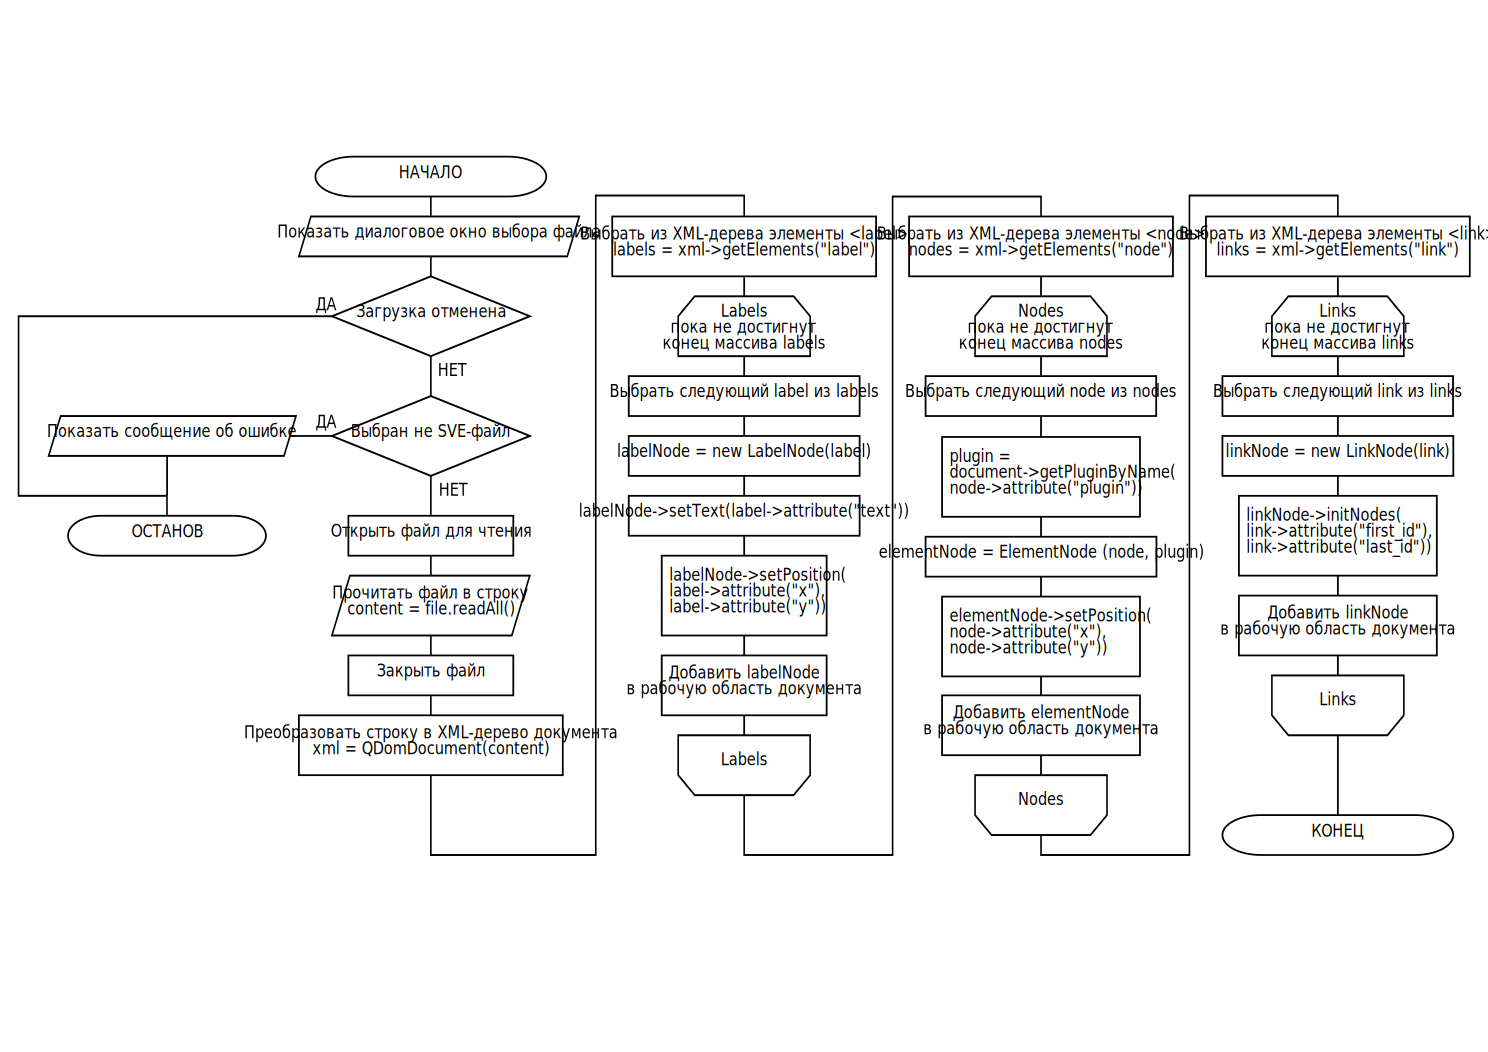
\includegraphics[width=0.55\textwidth]{gui/errors/load.png}
    \caption{Сообщение об ошибке при открытии документа несоответствующего типа}
  \end{figure}
  \item Используется поврежденное расширение.\\
  При попытке использования некорректного расширения система не прерывает своей работы, но игнорирует неверные расширения.
  \item Отствует файл настроек.\\
  Файл настроек или соответствующий раздел системного реестра может отсутствовать, если система впервые запускается на ЭВМ пользователя или если он был по той или иной причине удален.
  В случае отсутствия файла настроек система создаст его, заполнив стандартными значениями, и продолжит свою работу.
  \item В системе пользователя отсутствует GHDL.\\
  В этом случае при проверке исходного кода пользователю будет показано сообщение <<Ошибка запуска GHDL>>.
  \begin{figure}[H]
    \centering
    \includegraphics[width=0.95\textwidth]{gui/errors/ghdl.png}
    \caption{Сообщение об ошибке при отсутсвии GHDL}
  \end{figure}
  \item В процессе проверки исходного кода обнаружены ошибки.\\
  Если в процессе проверки исходного кода были обнаружены ошибки, сообщение об этом будет выведено в статусном поле окна просмотра VHDL.
  \begin{figure}[H]
    \centering
    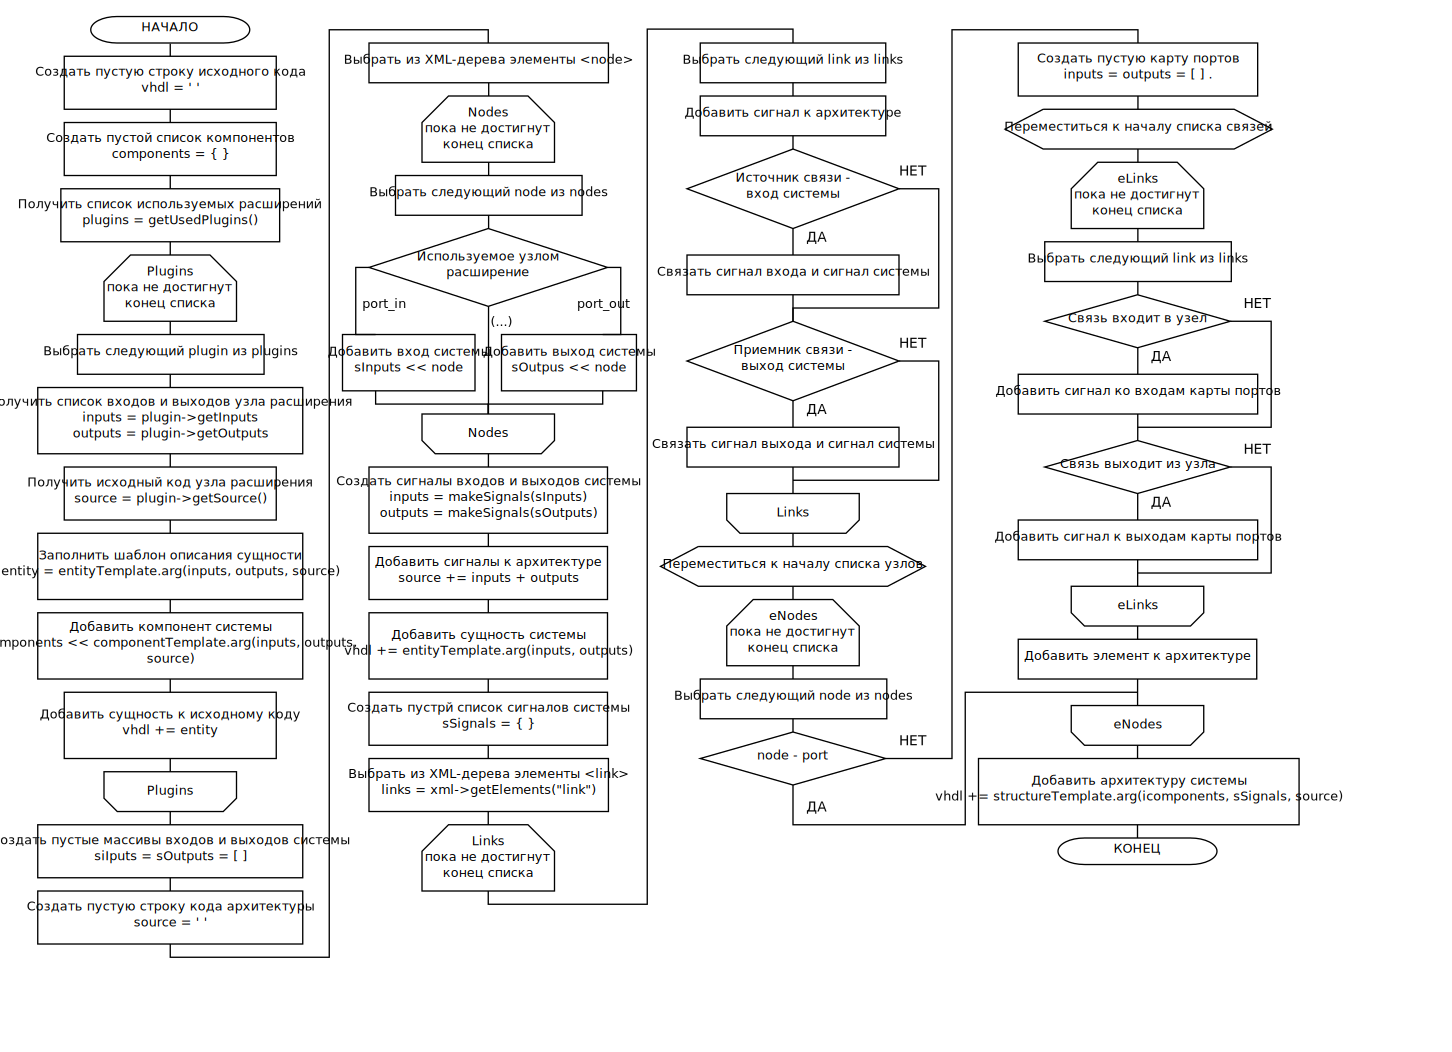
\includegraphics[width=0.95\textwidth]{gui/errors/vhdl.png}
    \caption{Сообщение об ошибке при проверке синтаксиса}
  \end{figure}
\end{itemize}